%This perspective should clarify how code or other artifacts come from idea into the running system and everything that happens on the way.

%In particular, the following descriptions should be included:

    %A complete description of stages and tools included in the CI/CD chains, including deployment and release of your systems.

    %How do you monitor your systems and what precisely do you monitor?

    %What do you log in your systems and how do you aggregate logs?

    %Brief results of the security assessment and brief description of how did you harden the security of your system based on the analysis.
    
    %Applied strategy for scaling and upgrades.
    
%In case you have used AI-assistants during your project briefly explain which system(s) you used during the project and reflect how it supported or hindered your process.



\section{Process' perspective}

\subsection{CI/CD Workflow}

\begin{figure}[H]
    \centering
    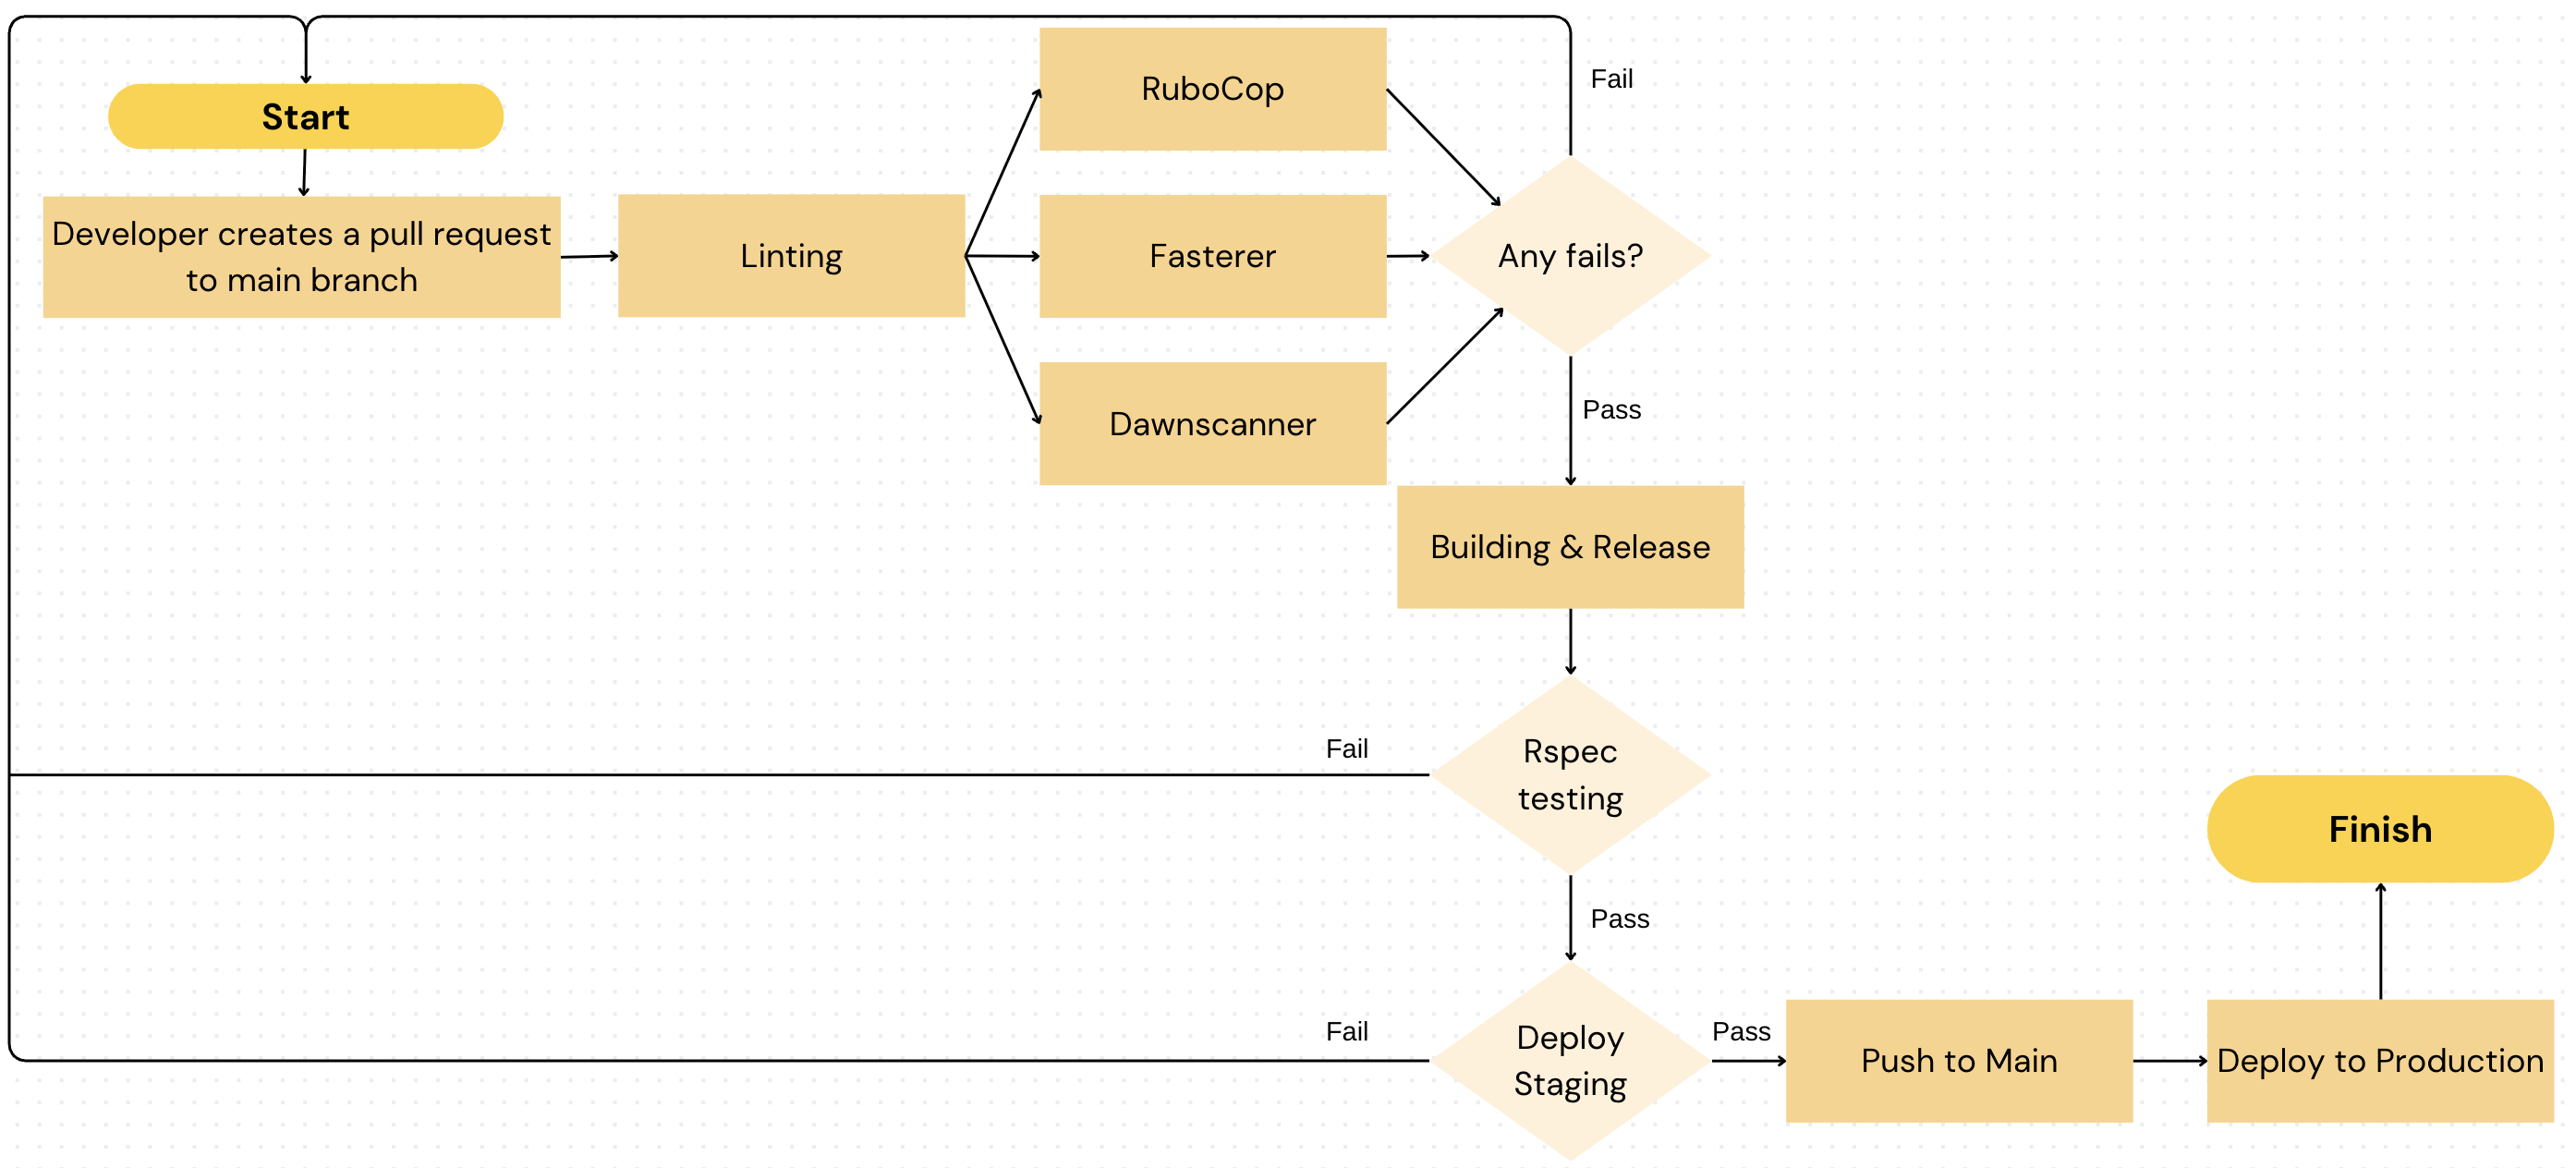
\includegraphics[width=1\linewidth]{images/Workflow.png}
    \caption{CI/CD workflow}
    \label{fig:Workflow}
\end{figure}
Figure~\ref{fig:Workflow} shows the overall CI/CD workflow. Our pipeline is implemented using GitHub Actions, which automates the process of linting, building, testing, and deploying the system upon each pull request to the \texttt{main} branch. 

\subsubsection{Continuous Integration: Test and Build}
Every pull request to \texttt{main} triggers the CI pipeline starting the linting tools. \texttt{RuboCop} Checks for style violations and enforces coding standards. It has the lowest risk but it also easier to fix as it suggests auto-fixes for most of the recommendations. \texttt{Fasterer} analyzes the code for inefficient patterns and suggests performance improvements. It is static and fast, but it’s focused on optimization, not correctness. It runs after style checks to catch possible refactors. \texttt{Dawnscanner} performs a static security audit, flagging potential vulnerabilities in our Ruby codebase. This is the most impactful check if vulnerabilities are found because security scans can be more computationally expensive and less frequent in early development, but critical before any merge or deploy. Finally, we also use SonarQube in our pipeline. This tool catches both security flaws and code smells, that could make our code less maintainable. \\

After passing all static analysis tools, our CI pipeline build the docker image an creates a release. The release is used for the unit and integration test. It runs \texttt{Rspec} to execute the test suite to ensure that our application logic is functioning as intended before moving on. If any \texttt{Rspec} test fails, the pipeline stops, and deployment is halted. This fail-fast strategy prevents broken code from reaching staging or production. 
The docker image build is later used for stage deployment(see section \ref{CD-sec}).

\subsubsection{Continuous Deployment}\label{CD-sec}

\begin{figure}[H]
    \centering
    
\includegraphics[width=1\linewidth]
    {images/CD.png}
    \caption{CD-Pipeline}
    \label{fig:CD}
\end{figure}

Figure~\ref{fig:CD} is the CD pipeline and illustrates how the staging works for the development environment and production. Our Continuous Deployment pipeline is defined as a GitHub Actions workflow triggered on pushes to the \texttt{main} branch. It performs automated end-to-end deployment using Docker and DigitalOcean Droplets. \\

After building Docker images for the web and database services using \texttt{docker compose}, the images are tagged and pushed to DockerHub. From there, the pipeline establishes SSH connections to two separate production servers: one for the PostgreSQL database, and one for the Ruby-based web application. \\

On the database server, the pipeline stops and removes existing containers, pulls the latest image, and redeploys the database using environment variables and persistent storage. \\

On the application server, the pipeline pulls the latest web image, runs Sequel database migrations, and then starts the application container with the required environment configuration. Finally, we use a curl-based HTTP check to verify the service is online. \\

This pipeline ensures fast, repeatable deployments and minimizes manual errors. We use secrets and environment variables to secure sensitive credentials and configuration data throughout the workflow.


\subsection{Monitoring}
To ensure the health, performance, and observability of our MiniTwit system, we implemented a multi-layered monitoring setup combining container health checks, application-level instrumentation, and Prometheus-based scraping.
For healthchecks we use Docker’s built-in healthcheck functionality to monitor the readiness of the PostgreSQL database. With a 5-second interval and 3-second timeout, retrying up to 5 times. This check ensures the database is reachable before the frontend service attempts to connect, which helps prevent runtime errors caused by timing issues during container startup. To make sure the application only starts once the database is healthy, the condition \texttt{service\_healthy} is used for improving stability in both development and deployment environments. \\

Our Ruby web application-level monitoring is implemented using the prometheus-client gem and a custom middleware \texttt{MetricsHelper} that captures \textbf{HTTP response counts}, labeled by status, HTTP method, and \textbf{request durations}, measured in milliseconds. These metrics are exposed via a /metrics endpoint in Prometheus text format, which Prometheus scrapes at regular intervals. \\

Our Prometheus is configured via prometheus.yml to scrape metrics from The webapp container and itself, \textbf{prometheus:9090} for internal health. We use 5-15 second scrape intervals for near real-time visibility.


\subsection{Logging}

We implemented logging using the ELFK stack. The stack helps us build and collect structured logs, that we can store and query, to get an overview of activity on the service. We have made a log-folder that lives in our docker containers, and is mounted in a droplet, to retain the data. The log-folder contains files like:

\begin{itemize}
    \item Debug
    \item Info
    \item Warning
    \item Error
    \item Fatal
    \item unknown
\end{itemize}

This structure helps us easily identify the best logs for finding and solving problems for debugging or optimization, or even just curiosity about what our users are doing on the site. We log things like status codes, http requests, and timestamps. Kibana creates visualizations across the log-files. \\


\subsection{Security}
When looking at our security, our main assets are the containers, that are exposed to the internet. This is both the webapp, the monitoring system, the logging system and the database. However, monitoring, logging and the database, only expose specific ports, and are password protected. This ensures that our data cannot be seen and modified by malicious actors.\\

The web application interacts with the database using an ORM layer, 'Sequel' in our case, which helps mitigate SQL injection by ensuring proper query parameterization. Similarly, the templating system used for rendering HTML, 'Embedded Ruby - .erb' in our case, escapes user input by default, which protects against common Cross-Site Scripting (XSS) attacks. \\

To keep sensitive environment variables, like access-tokens, passwords and private keys, secure, we use GitHub secrets. This way, we can store secrets, and use them in workflows, without exposing them to the world, in our repository. 


\subsection{Scaling and reliability}
To improve scalability and reliability for our application, we utilize Docker Swarm. Docker Swarm allows us to define a logic for managing Docker containers, like how they share/sync data between them, or if they simply have a central database and leader-node, as is the case for us.\\

In our setup, we maintain a central PostgreSQL database hosted on a dedicated, isolated Droplet, while the application containers are managed from another central Droplet. \\

Swarm provides automatic load balancing by distributing incoming requests across available replicated containers. It also offers fault tolerance by rescheduling affected services elsewhere in the cluster, if a container crashes or becomes unavailable. This orchestration simplifies scaling and improves the robustness of our deployment.
